\documentclass[tikz,border=10pt]{standalone}
\usepackage[T1]{fontenc}
\usepackage{lmodern}
\usetikzlibrary{arrows.meta,backgrounds,positioning,shapes.geometric}

\definecolor{ink}{HTML}{172033}
\definecolor{muted}{HTML}{59697F}
\definecolor{panel}{HTML}{F8FAFC}
\definecolor{panelborder}{HTML}{DCE5F0}
\definecolor{purple}{HTML}{7138E8}
\definecolor{purplefill}{HTML}{F0ECFF}
\definecolor{blue}{HTML}{2563EB}
\definecolor{bluefill}{HTML}{E1EDFF}
\definecolor{green}{HTML}{169B45}
\definecolor{greenfill}{HTML}{E1FBEA}
\definecolor{amber}{HTML}{D97706}
\definecolor{amberfill}{HTML}{FFF3C4}
\definecolor{red}{HTML}{C2410C}
\definecolor{redfill}{HTML}{FFF0E8}

\tikzset{
  flow/.style={-{Latex[length=2.7mm,width=2.1mm]},draw=muted,line width=1.05pt,rounded corners=3pt},
  agent/.style={draw=purple,fill=purplefill,line width=1.1pt,rounded corners=4pt,minimum width=36mm,minimum height=14mm,align=center,inner sep=3pt},
  tool/.style={draw=blue,fill=bluefill,line width=1.1pt,rounded corners=4pt,minimum width=42mm,minimum height=14mm,align=center,inner sep=3pt},
  passive/.style={draw=green,fill=greenfill,line width=1.1pt,rounded corners=4pt,minimum width=42mm,minimum height=14mm,align=center,inner sep=3pt},
  decision/.style={diamond,aspect=1.65,draw=amber,fill=amberfill,line width=1.1pt,minimum width=25mm,minimum height=17mm,align=center,inner sep=1pt},
  count decision/.style={decision,minimum width=31mm,minimum height=20mm},
  stop/.style={draw=red,fill=redfill,line width=1.1pt,rounded corners=4pt,minimum width=36mm,minimum height=14mm,align=center,inner sep=3pt},
  context/.style={draw=panelborder,fill=white,line width=1.0pt,minimum width=42mm,minimum height=14mm,align=center,inner sep=3pt},
  edge label/.style={fill=panel,inner sep=2pt,font=\sffamily\bfseries\small,text=muted}
}

\begin{document}
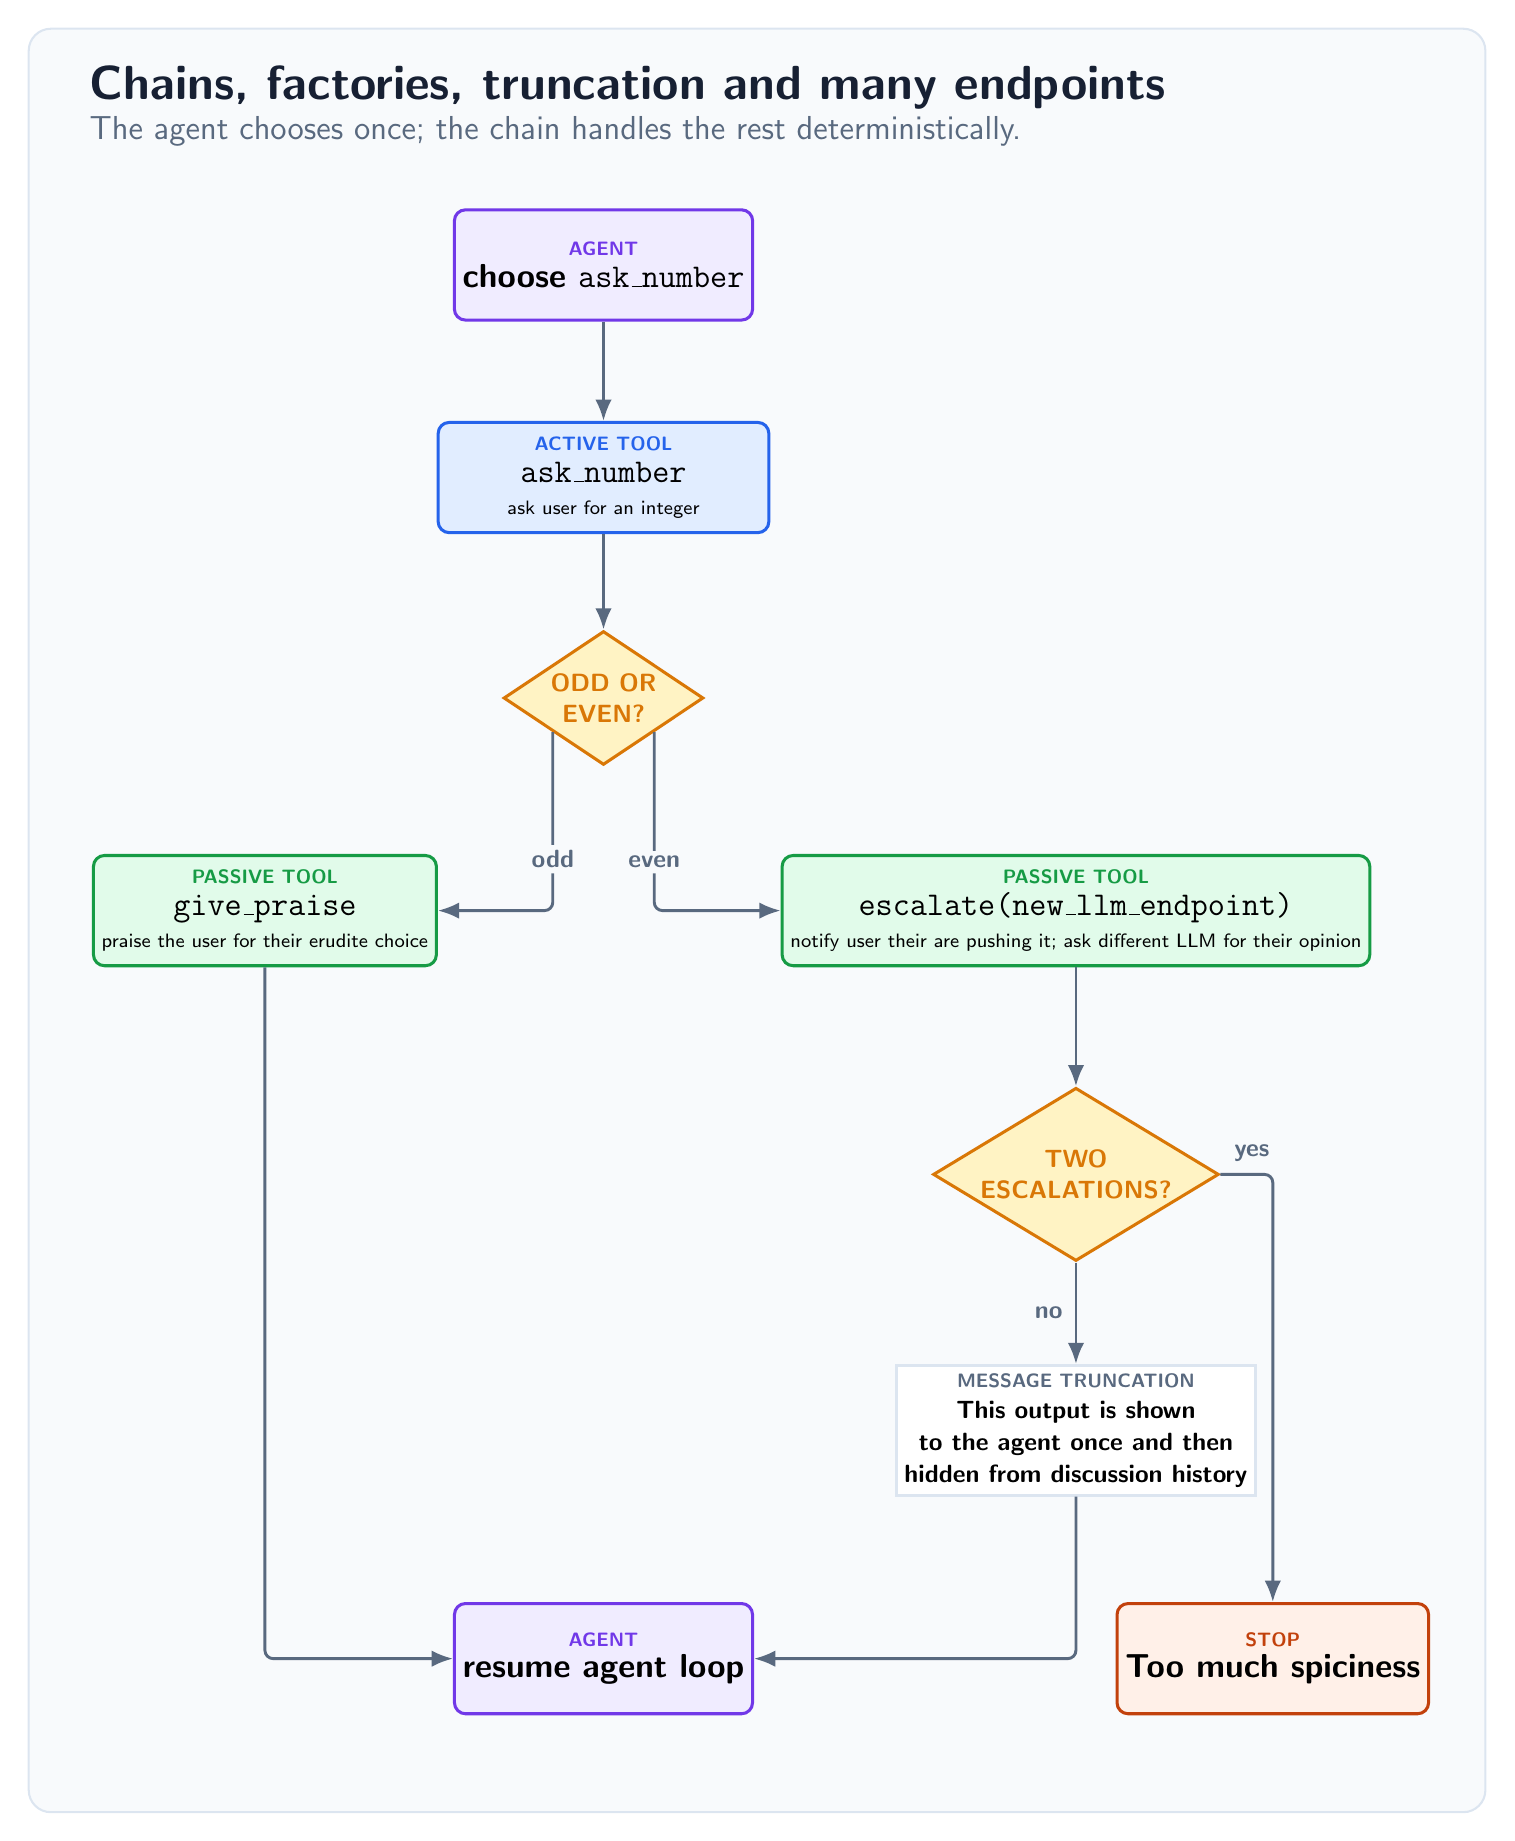
\begin{tikzpicture}[font=\sffamily]
  \begin{scope}[on background layer]
    \draw[draw=panelborder,fill=panel,line width=0.75pt,rounded corners=8pt]
      (-7.3,2.45) rectangle (11.2,-20.2);
  \end{scope}

  \node[anchor=west,font=\sffamily\bfseries\LARGE,text=ink] at (-6.65,1.7)
    {Chains, factories, truncation and many endpoints};
  \node[anchor=west,font=\sffamily\large,text=muted] at (-6.65,1.15)
    {The agent chooses once; the chain handles the rest deterministically.};

  \node[agent] (agent) at (0,-0.55) {
    {\scriptsize\bfseries\color{purple}AGENT}\\[-0.2mm]
    {\large\bfseries choose \texttt{ask\_number}}
  };
  \node[tool] (ask) at (0,-3.25) {
    {\scriptsize\bfseries\color{blue}ACTIVE TOOL}\\[-0.2mm]
    {\large\bfseries \texttt{ask\_number}}\\[-0.2mm]
    {\scriptsize ask user for an integer}
  };
  \node[decision] (parity) at (0,-6.05) {
    {\small\bfseries\color{amber}ODD OR}\\[-0.3mm]
    {\small\bfseries\color{amber}EVEN?}
  };

  \node[passive] (praise) at (-4.3,-8.75) {
    {\scriptsize\bfseries\color{green}PASSIVE TOOL}\\[-0.2mm]
    {\large\bfseries \texttt{give\_praise}}\\[-0.2mm]
    {\scriptsize praise the user for their erudite choice}
  };
  \node[passive] (escalate) at (6,-8.75) {
    {\scriptsize\bfseries\color{green}PASSIVE TOOL}\\[-0.2mm]
    {\large\bfseries \texttt{escalate(new\_llm\_endpoint)}}\\[-0.2mm]
    {\scriptsize notify user their are pushing it; ask different LLM for their opinion}
  };
  \node[count decision] (count) at (6,-12.1) {
    {\small\bfseries\color{amber}TWO}\\[-0.3mm]
    {\small\bfseries\color{amber}ESCALATIONS?}
  };
  \node[context] (visible-once) at (6,-15.35) {
    {\scriptsize\bfseries\color{muted}MESSAGE TRUNCATION}\\[-0.2mm]
    {\small\bfseries This output is shown}\\[-0.2mm]
    {\small\bfseries to the agent once and then}\\[-0.2mm]
    {\small\bfseries hidden from discussion history}
  };
  \node[stop] (stop) at (8.5,-18.25) {
    {\scriptsize\bfseries\color{red}STOP}\\[-0.2mm]
    {\large\bfseries Too much spiciness}
  };
  \node[agent] (resume) at (0,-18.25) {
    {\scriptsize\bfseries\color{purple}AGENT}\\[-0.2mm]
    {\large\bfseries resume agent loop}
  };

  \draw[flow] (agent.south) -- (ask.north);
  \draw[flow] (ask.south) -- (parity.north);
  \draw[flow] (parity.south west) -- ++(0,-1.1) |- node[edge label,pos=0.34,above=0.8mm] {odd} (praise.east);
  \draw[flow] (parity.south east) -- ++(0,-1.1) |- node[edge label,pos=0.34,above=0.8mm] {even} (escalate.west);
  \draw[flow] (praise.south) |- (resume.west);
  \draw[flow] (escalate.south) -- (count.north);
  \draw[flow] (count.south) -- node[edge label,left=0.8mm] {no} (visible-once.north);
  \draw[flow] (visible-once.south) |- (resume.east);
  \draw[flow] (count.east) -| node[edge label,pos=0.3,above=0.8mm] {yes} (stop.north);
\end{tikzpicture}
\end{document}
